\PassOptionsToPackage{activate=false,babel=false}{microtype}
\documentclass[sigplan,screen]{acmart}

\usepackage{mathpartir}
\usepackage{algorithm}
\usepackage{algpseudocode}
\usepackage{amsmath}
\usepackage{amssymb}
\usepackage{xspace}
\usepackage{tikz}
\usetikzlibrary{decorations.pathreplacing,arrows.meta,positioning}

%% ---- Custom commands ----
%% Reference to a Lean 4 artifact
\newcommand{\leanref}[1]{\texttt{#1}}

%% Multi-letter math identifiers
\newcommand{\YjsLt}{\mathrel{<_Y}}
\newcommand{\YjsLeq}{\mathrel{\leq_Y}}
\newcommand{\hb}{\mathrel{\prec}}
\newcommand{\hble}{\mathrel{\preceq}}
\newcommand{\CC}{\mathit{CC}}

%% Semantic domains
\newcommand{\First}{\mathsf{first}}
\newcommand{\Last}{\mathsf{last}}
\newcommand{\OriginLt}{\mathrel{<_{\mathit{orig}}}}

%% BNF helpers
\newcommand{\bnfdef}{\;::=\;}
\newcommand{\bnfmid}{\;\mid\;}

%% Named sets / functions
\newcommand{\interpOps}{\mathit{interpOps}}
\newcommand{\effect}{\mathit{effect}}
\newcommand{\init}{\mathit{init}}
\newcommand{\histories}{\mathcal{H}}
\newcommand{\Deliver}{\mathsf{Deliver}}
\newcommand{\Broadcast}{\mathsf{Broadcast}}
\newcommand{\Delivered}[1]{\mathit{delivered}_{#1}}
%% Kleisli composition of partial functions (used for Gomes commutativity)
\newcommand{\kleisli}{\mathbin{\triangleright}}

\copyrightyear{2025}
\acmYear{2025}

\author{Izumi Asakura}
\email{i.asakura58@gmail.com}

\begin{document}

\title{Conditional Commutativity: A Generic Convergence Proof for
  CRDTs and Its Application to Yjs}

\begin{abstract}
Operation-based CRDTs are typically proved correct by showing that
concurrent operations commute, possibly under enabledness or delivery
preconditions.  Existing mechanized convergence frameworks, such as that of
Gomes~et~al., side-step the precondition obligation by requiring
\emph{unconditional} commutativity; this approach does not extend to Yjs,
whose insert effector is well-defined only on states satisfying a
structural invariant.  We exhibit a mechanized counterexample in Lean~4
witnessing the failure of unconditional commutativity for Yjs, and propose
a generic \emph{prefix-level conditional commutativity} framework: a
convergence theorem that requires commutativity only on invariant-satisfying
states and combines it with a prefix-level causal validity transport
condition.  The latter is a mechanized refinement of the
delivery-precondition obligation already implicit in the Shapiro-style
op-based CRDT theorem.  We instantiate the framework for Yjs, obtaining the first
complete machine-checked proof that the Yjs core CRDT algorithm achieves
strong eventual consistency.  The entire development is formalized in
Lean~4 with no axioms beyond those of its type theory.
\end{abstract}

\maketitle

%%
%% -------------------------------------------------------------------
\section{Introduction}
\label{sec:intro}
%%

%% P1: Motivation
Collaborative editors must reconcile edits like insertions and deletions
of characters performed at different replicas without requiring a single
global order of user actions.  Conflict-free replicated data types
(CRDTs)~\cite{Shapiro2011} are a class of data structures designed for
this style of replication, in which each replica processes operations
locally and replicas converge to the same state once they have exchanged
all updates.  Yjs~\cite{Yjs2023} is one of the most widely deployed CRDT
implementations for sequence data, powering collaborative editors such as
Tiptap~\cite{TipTap2024}.  Its core algorithm is intricate, however, and
reasoning about its correctness by hand is error-prone.  Indeed, we
discovered a non-convergent case in the pseudocode published in the YATA
paper of Nicolaescu et al.~\cite{Nicolaescu2016} on which Yjs is based.  The original author
confirmed our finding, remarking that ``Nine years later, you are
actually the first to point out the issue in the pseudocode in the
paper''~\cite{YjsBugDiscussion2024}.  The fact that the issue went
unnoticed for nine years illustrates why machine-checked correctness
proofs are valuable for CRDTs of this complexity.

%% P2: Prior work on Yjs correctness
To the best of our knowledge, no complete machine-checked convergence
proof has been published for the Yjs core algorithm.  Among prior work
formally arguing the correctness of Yjs, Nicolaescu et
al.~\cite{Nicolaescu2016} introduced YATA together with hand proofs of
selected properties, and Weidner et al.'s Fugue~\cite{Weidner2023}, a
closely related sequence CRDT, includes a by-hand proof for a variant
of the Yjs insertion procedure in its appendix.  Both efforts
remain at the level of proof sketches and leave significant gaps to a
complete formalization.

%% P3: Gomes framework
Gomes et al.~\cite{Gomes2017} proposed a formal verification framework
for operation-based CRDTs.  They give a network model of op-based CRDT,
a commutativity-based convergence theorem, and instantiate them to
verify several CRDT algorithms including RGA~\cite{Roh2011}, a simpler list CRDT than Yjs.
Deriving convergence (strong eventual consistency) from commutativity of concurrent
operations is the standard verification method for op-based CRDTs.
The Gomes framework formalizes this method by providing a convergence
theorem that says commutativity of all concurrent operation pairs on
arbitrary state suffices to obtain convergence.

%% P4: Why Gomes does not apply to Yjs
However, as we show in \S\ref{sec:overview}, the Gomes framework cannot
be applied to Yjs, because Yjs is not commutative in the sense the
framework requires.  In that definition, commutativity is
$\effect(a, \effect(b, s)) = \effect(b, \effect(a, s))$ for every
concurrent pair of operations $a$, $b$ and every state $s$, where
$\effect$ applies an operation (e.g., an insert) to a state (e.g., a
list).  Yjs
operations commute only when the operations and the state satisfy a
specific structural condition.  Since Gomes's definition gives the
operations and the state independently, such a relational constraint
cannot be expressed.  In this work we prove a convergence theorem under
a relaxed commutativity, which we call \emph{conditional commutativity},
and use it to obtain the first complete machine-checked proof of strong
eventual consistency for the Yjs core CRDT algorithm
(Theorem~\ref{thm:yjs-convergence}).

%% P5: Our solution — proving commutativity for Yjs
We prove commutativity by defining a strict total order on Yjs items
and showing that every Yjs operation preserves the invariant that the
array is sorted under this order; since a strict total order admits at
most one sorted arrangement of any item set, two delivery orders
producing the same item set produce identical arrays.  The overall
strategy is the same as Nicolaescu et al.~\cite{Nicolaescu2016}, but
the order definition and the preservation proof are new.  Our order is
derived from the conditions intuitively required of any Yjs-compatible
order, yet strong enough to be a strict total order.  Insert
preservation is proved by a loop invariant with intricate conditions,
and its preservation step reasons about six independent cases
determined by the algorithm's branch and the loop's scanning state.
The order definition, the loop invariant, and the six-case
preservation analysis are all machine-checked in Lean~4, ruling out
the case omissions to which informal correctness proofs of such
intricate algorithms are prone.

%% P6: Contributions
This work makes two contributions.
\begin{enumerate}
\item \textbf{A prefix-level conditional commutativity framework.}
  We formulate, and mechanize in Lean~4, a reusable convergence theorem
  for operation-based CRDTs whose effectors are state-dependent.  The
  theorem requires commutativity only when both concurrent operations are
  valid at the current state, together with a prefix-level causal
  validity transport condition ensuring that broadcast-time validity
  survives any causally compatible reordering of the delivery list.
  This may be viewed as a mechanized, prefix-level refinement of the
  delivery-precondition obligation implicit in Shapiro-style op-based CRDTs,
  while generalizing the unconditional-commutativity convergence theorem
  used by Gomes et al.  We accompany the framework with a mechanized
  counterexample showing that unconditional commutativity is genuinely
  too strong for Yjs.
\item \textbf{First formal verification of the Yjs core CRDT algorithm.}
  We instantiate the generic framework for Yjs, providing the first
  machine-checked proof that the core algorithm achieves strong eventual
  consistency.  Our main lemma is the preservation of the total order on
  items by the Yjs insert and delete operations.  The insert operation,
  in particular, is defined by a non-trivial procedural loop, and proving
  that it preserves the order required discovering a four-part loop
  invariant.  We also mechanize a strict total order on Yjs items, satisfying
  totality, transitivity, and asymmetry, together with a no-cross-origin
  lemma that drives the preservation proof.  The inference rules of the
  order are carefully balanced so that transitivity and asymmetry can be
  recovered via size-based induction.
\end{enumerate}

%% P7: Paper organization
Section~\ref{sec:definitions} defines the network model and Yjs data
structures.
Section~\ref{sec:overview} presents the counterexample motivating
conditional commutativity and gives an overview of the proof architecture.
Sections~\ref{sec:order}--\ref{sec:convergence} develop the proof.
Section~\ref{sec:related} discusses related work, and
Section~\ref{sec:conclusion} concludes.
Detailed proofs for the order-theoretic properties appear in
Appendix~\ref{app:order-proofs}.

%%
%% -------------------------------------------------------------------
\section{Network and Execution Model}
\label{sec:definitions}
%%

This section presents the network model and its instantiation to Yjs.  We
first introduce a generic operation network model, a mild reformulation of
the OOPSLA'17 framework of Gomes et al.~\cite{Gomes2017}, parameterized by
a message type, an operation structure (state space, initial state, and
effect function), and a validity predicate.  We then define the Yjs
execution model by instantiating each parameter with Yjs-specific data
structures and operations, and finally state the main convergence theorem.

%%
\subsection{Network Model}
\label{subsec:network}
%%

A network is a family of replicas, each maintaining a local sequence of
events that records the \emph{broadcast} of a locally issued operation and
the \emph{deliver} events at which operations are applied to the local
state.  Broadcasts disseminate operations to other replicas; only deliver
events change the local state.  On top of this bare structure we impose a
Lamport-style causality condition~\cite{Lamport1978}, then equip operations
with a transition semantics and a validity predicate.

%% P1: Messages, Events, Node Histories, Local Ordering
The model is parameterized by a message type~$A$.
Each message $m \in A$ carries an identifier $\mathit{msgId}(m) \in M$
that uniquely determines it.

\begin{definition}[Event (\leanref{Event})]\label{def:event}
An \emph{event} is either the broadcast or delivery of a message:
\[
  e \bnfdef \Broadcast(m) \bnfmid \Deliver(m)
\]
\end{definition}

\begin{definition}[Node history (\leanref{NodeHistories})]\label{def:node-history}
A \emph{node history} $H_i$ for node $i \in \mathbb{N}$ is a duplicate-free
list of events.  For events $e_1, e_2 \in H_i$ we write $e_1 <_i e_2$
(\emph{locally ordered}) when $e_1$ appears before $e_2$ in $H_i$.
\end{definition}

%% P2: Network, Happens-Before, Causal Network
\begin{definition}[Network (\leanref{NetworkBase})]\label{def:network-base}
A \emph{network} is a family of node histories
$\{H_i \mid i \in \mathbb{N}\}$ satisfying the following properties:
\begin{itemize}
\item[(N1)] Every delivered message has a broadcasting node:
  $\Deliver(m) \in H_i \Rightarrow \exists j.\; \Broadcast(m) \in H_j$.
\item[(N2)] Broadcast precedes delivery locally:
  $\Deliver(m) \in H_i \Rightarrow \Broadcast(m) <_i \Deliver(m)$.
\item[(N3)] Message IDs are globally unique:
  if $\Broadcast(m_1) \in H_i$, $\Broadcast(m_2) \in H_j$, and
  $\mathit{msgId}(m_1) = \mathit{msgId}(m_2)$, then
  $\Broadcast(m_1) = \Broadcast(m_2)$.
\end{itemize}
\end{definition}

Operation-based CRDTs rely on a \emph{causal network}: the network is
required to deliver messages in an order that respects the happens-before
relation of Lamport~\cite{Lamport1978}, so that every message encounters
its causal predecessors before delivery.  Formally, we extend
Definition~\ref{def:network-base} as follows.

\begin{definition}[Happens-before (\leanref{HappensBefore})]\label{def:happens-before}
The \emph{happens-before} relation $\hb$ is the least relation satisfying:
\begin{mathpar}
\inferrule*[right=HB-Local-Bc]
  {\Broadcast(m_1) <_i \Broadcast(m_2)}
  {m_1 \hb m_2}
\and
\inferrule*[right=HB-Deliver]
  {\Deliver(m_1) <_i \Broadcast(m_2)}
  {m_1 \hb m_2}
\and
\inferrule*[right=HB-Trans]
  {m_1 \hb m_2 \\ m_2 \hb m_3}
  {m_1 \hb m_3}
\end{mathpar}
\end{definition}

\begin{definition}[Causal network (\leanref{CausalNetwork})]\label{def:causal-network}
A \emph{causal network} extends a network with the property that if
$m_2$ is delivered at node~$i$ and $m_1 \hb m_2$, then $\Deliver(m_1) <_i
\Deliver(m_2)$.
\end{definition}

%% P3: Operation, Operation Network, Delivered Messages, Interpretation
So far, the message type~$A$ only carries an identifier.
An \emph{operation network} equips messages with additional structure: a
state-transition semantics and a validity predicate, so that messages can be
interpreted as state-transforming operations.  We first define the
state-transition structure, then introduce the delivered-message projection
that turns a history into the sequence of operations that actually affect
state, and finally the validity predicate.

\begin{definition}[Operation (\leanref{Operation})]\label{def:operation}
An \emph{operation structure} on a message type~$A$ is a tuple
$(\mathit{St},\; \init,\; \effect)$ where
$\mathit{St}$ is the set of states,
$\init \in \mathit{St}$ is the initial state, and
$\effect : A \to \mathit{St} \to \mathit{St}_\bot$ is a partial effect
function; here $\mathit{St}_\bot = \mathit{St} \sqcup \{\bot\}$ is the
disjoint sum of $\mathit{St}$ with a single failure value $\bot$.\footnote{In
the Lean~4 artifact the failure value carries a string error message
(\leanref{Err}); we omit this detail here because the error payload plays no
role in the proofs.}
\end{definition}
\noindent
We write $\interpOps(ms, s)$ for the result of folding $\effect$ over a
message list~$ms$ starting from state~$s$, and
$\Delivered{i}(H_i)$ for the sublist of $H_i$ consisting of all $\Deliver$
events projected to their message payloads.  Because broadcasts have no
effect, the local state at node~$i$ after running the history $H_i$ is
precisely $\interpOps(\Delivered{i}(H_i),\, \init)$.

\begin{definition}[Operation network (\leanref{OperationNetwork})]\label{def:operation-network}
An \emph{operation network} extends a causal network whose message type~$A$
is equipped with both an operation structure
(Definition~\ref{def:operation}) and a validity predicate
$\mathit{isValid} : \mathit{St} \to A \to \mathit{Prop}$, subject to the
following condition.
\begin{itemize}
\item[(V)] \emph{Broadcast validity.}  Whenever
$H_i = \mathit{pre} \mathbin{+\!\!+}
[\Broadcast(m)] \mathbin{+\!\!+} \mathit{post}$ for some prefix
$\mathit{pre}$ and suffix $\mathit{post}$, there exists a state $s$
such that $\interpOps(\Delivered{i}(\mathit{pre}), \init) = s$ and
$\mathit{isValid}(s, m)$ holds.
\end{itemize}
\end{definition}
\noindent
Condition~(V) is intentionally weaker than the prefix-level causal validity
condition introduced in \S\ref{sec:convergence}: it records that a message
was well-formed when it was issued, but it does not by itself imply that
the same message remains valid at the intermediate states encountered by a
swap-based commutativity proof.

%%
\subsection{Yjs Data Model}
\label{subsec:yjs-data}
%%

We now define the data structures and algorithms that constitute the Yjs
core CRDT.  We restrict our attention to the core insert and delete
operations on a sequence of \emph{items}, each recording the neighbors it
was inserted between (its \emph{origin} and \emph{right-origin}).  We make
no attempt to model garbage collection, undo/redo, subdocuments, or the
awareness protocol of the Yjs manual~\cite{Yjs2023}.

%% P4: YjsPtr, YjsItem (with YjsId merged in)
Each item records its left and right neighbors at the moment of the
originating broadcast; we use the sentinels $\First$ and $\Last$ at the
document boundary.

\begin{definition}[Yjs pointer and item (\leanref{YjsPtr}, \leanref{YjsItem})]
\label{def:yjs-item}
\emph{Yjs pointers}~$p$ and \emph{Yjs items}~$x$ are defined by mutual
recursion:
\begin{align*}
  p &\bnfdef \First \bnfmid \Last \bnfmid \langle x \rangle \\
  x &\bnfdef \{
    \mathit{origin} : p,\;
    \mathit{rightOrigin} : p,\;
    \mathit{id} : \mathit{YjsId},\;
    \mathit{content} : A \}
\end{align*}
where $\mathit{YjsId} = \mathit{ClientId} \times \mathbb{N}$ is the
identifier type, pairing a client identifier with a logical clock and
compared lexicographically.\footnote{The real Yjs implementation
references $\mathit{origin}$ and $\mathit{rightOrigin}$ by identifier; we
embed items directly inside pointers for proof convenience.  The artifact
contains an \emph{indirect} variant (\texttt{LeanYjs/Indirect}) that
follows the implementation faithfully and proves it equivalent to the
direct definition used here, so convergence transports automatically.}
\end{definition}

%% P5: YjsState, deletion
\begin{definition}[Yjs state (\leanref{YjsState})]\label{def:yjs-state}
A \emph{Yjs state} consists of an array of all items inserted so far
(including those that have since been deleted) together with a set of
deleted identifiers:
\[
  \mathit{YjsState}(A) = \{
    \mathit{items} : \mathit{Array}(\mathit{YjsItem}(A)),\;
    \mathit{deletedIds} : \mathit{Set}(\mathit{YjsId}) \}
\]
Deletion is implemented logically via tombstones: the deleted identifier is
added to $\mathit{deletedIds}$ while the item remains in the array, preserving
the anchor points needed by subsequent insertions.
\end{definition}

%%
\subsection{Yjs as an Operation Network Instance}
\label{subsec:yjs-network}
%%

We define the Yjs execution model by instantiating the generic operation
network of \S\ref{subsec:network}: we give the message type, its
operation structure, and the validity predicate, and additionally impose
two Yjs-specific well-formedness properties on how clients issue
broadcasts.

%% P6: YjsOperation, Effect, Insert Algorithm, YjsOperationNetwork
\begin{definition}[Yjs operation (\leanref{YjsOperation})]\label{def:yjs-operation}
A \emph{Yjs operation} either inserts a new item or marks an existing one as
deleted:
\begin{align*}
  \mathit{op} &\bnfdef \mathsf{Insert}(\mathit{inp})
                \bnfmid \mathsf{Delete}(\mathit{id},\, \mathit{deletedId}) \\
  \mathit{inp} &\bnfdef \{
    \mathit{originId} : \mathit{YjsId},\;
    \mathit{rightOriginId} : \mathit{YjsId},\; \\
  &\qquad\; \mathit{content} : A,\;
    \mathit{id} : \mathit{YjsId} \}
\end{align*}
where $\mathit{inp}$ is an \emph{insert input} recording the identifiers of
the origin and right-origin neighbors, the content, and the new item's
identifier.  This instantiates Definition~\ref{def:operation} with
$\mathit{St} = \mathit{YjsState}$,
$\mathit{init} = ([\,],\; \emptyset)$, and
\[
  \effect(\mathit{op},\, \sigma) \;=\;
  \begin{cases}
    \mathit{insert}(\sigma,\, \mathit{inp})
      & \text{if } \mathit{op} = \mathsf{Insert}(\mathit{inp}) \\
    \mathit{deleteById}(\sigma,\, \mathit{did})
      & \text{if } \mathit{op} = \mathsf{Delete}(\mathit{id},\, \mathit{did})
  \end{cases}
\]
Deletion simply adds $\mathit{did}$ to the tombstone set, so it always
succeeds.  Insertion is defined by Algorithm~\ref{alg:integrate}: starting
from the origin, the scan walks rightward through the existing items,
comparing each encountered item against the new one using the order
developed in \S\ref{sec:order}, and inserts the new item at the first
position where no conflicting item precedes it.  The detailed invariant
maintained by the loop is analyzed in \S\ref{sec:algorithm}.
\end{definition}

\begin{algorithm}[t]
\caption{Yjs insert algorithm}\label{alg:integrate}
\begin{algorithmic}[1]
\Require{insert input $\mathit{inp}$, items array $\mathit{arr}$}
\State $\mathit{leftIdx} \gets \mathit{findIndex}(\mathit{inp.originId},\, \mathit{arr})$
\Comment{$-1$ if origin is $\First$}
\State $\mathit{rightIdx} \gets \mathit{findIndex}(\mathit{inp.rightOriginId},\, \mathit{arr})$
\Comment{$|\mathit{arr}|$ if right-origin is $\Last$}
\State $\mathit{dest} \gets \mathit{leftIdx} + 1$
\State $\mathit{scanning} \gets \mathbf{false}$
\For{$i \gets \mathit{leftIdx}+1$ \textbf{to} $\mathit{rightIdx}-1$}
  \State $\mathit{other} \gets \mathit{arr}[i]$
  \State $\mathit{oLeft} \gets \mathit{findIndex}(\mathit{other.origin},\, \mathit{arr})$
  \State $\mathit{oRight} \gets \mathit{findIndex}(\mathit{other.rightOrigin},\, \mathit{arr})$
  \If{$\mathit{oLeft} < \mathit{leftIdx}$}
    \State \textbf{break}
  \ElsIf{$\mathit{oLeft} = \mathit{leftIdx}$}
    \If{$\mathit{inp.clientId} > \mathit{other.clientId}$}
      \State $\mathit{scanning} \gets \mathbf{false}$
    \ElsIf{$\mathit{oRight} = \mathit{rightIdx}$}
      \State \textbf{break}
    \Else
      \State $\mathit{scanning} \gets \mathbf{true}$
    \EndIf
  \EndIf
  \If{$\neg\, \mathit{scanning}$}
    \State $\mathit{dest} \gets i + 1$
  \EndIf
\EndFor
\State \Return $\mathit{arr}.\mathit{insert}(\mathit{dest},\, \mathit{mkItem}(\mathit{inp}, \mathit{arr}))$
\end{algorithmic}
\end{algorithm}

It remains to describe how Yjs clients issue broadcasts.  Yjs assigns
each client a unique identifier, and a single client tags its successive
broadcasts with strictly increasing clocks; both assumptions are honored
by every faithful implementation, and together they make item identifiers
globally unique.  We package these assumptions into the following
definition.

\begin{definition}[Yjs operation network (\leanref{YjsOperationNetwork})]\label{def:yjs-op-network}
A \emph{Yjs operation network} is an operation network on the Yjs operation
type satisfying the following Yjs-specific properties on broadcasts:
\begin{itemize}
\item[(Y1)] \textbf{Client ID consistency.} Every operation broadcast by node
  $i$ carries client ID $i$.
\item[(Y2)] \textbf{Clock monotonicity.} The clock component of the
  identifiers broadcast by a single client is strictly increasing along the
  local history.
\end{itemize}
\end{definition}

%%
\subsection{Main Theorem}
\label{subsec:main-theorem}
%%

%% P7
We can now state the main convergence result.

\begin{theorem}[Yjs Convergence, \leanref{YjsOperationNetwork\_converge'}]
\label{thm:convergence}
For any Yjs operation network and any two nodes $i$, $j$, if
$\Delivered{i}(H_i) \approx \Delivered{j}(H_j)$ (equality as sets), then
$\interpOps(\Delivered{i}(H_i), \init) =
 \interpOps(\Delivered{j}(H_j), \init)$.
\end{theorem}

\noindent
Here $\approx$ denotes that the two lists contain the same set of messages;
the ordering may differ.  That is, any two nodes that have delivered the same
set of operations converge to equal states.

%%
%% -------------------------------------------------------------------
\section{Overview of the Proof}
\label{sec:overview}
%%

This section presents the high-level structure of our convergence proof.
We first recall the convergence framework of Gomes et al.~\cite{Gomes2017}
and exhibit a Yjs counterexample showing that one of its
hypotheses, namely unconditional concurrent commutativity, is too strong for
Yjs (\S\ref{subsec:why-gomes}).  We then describe the generalization that
underlies our proof: conditional commutativity together with a causal
validity transport condition (\S\ref{subsec:our-approach}).

\subsection{Why Gomes et al.\ does not apply to Yjs}
\label{subsec:why-gomes}

The Gomes et al.\ Isabelle/HOL framework~\cite{Gomes2017} establishes
strong eventual consistency for an operation-based CRDT under the
following \emph{unconditional} commutativity premise: for every pair of
concurrent operations $a$ and $b$,
\[
  \hat{a} \kleisli \hat{b} \;=\; \hat{b} \kleisli \hat{a},
\]
where $\hat{x} \triangleq \lambda s.\,\effect(x, s)$ and $\kleisli$
denotes Kleisli composition of partial functions
($f \kleisli g \triangleq \lambda s.\, f(s) \mathbin{>\!\!>\!=} g$).
Once this property is verified for the CRDT under study, the framework
combines it with the causal-network axioms of \S\ref{subsec:network} to
conclude that any two nodes that have delivered the same set of
operations reach equal states.  The proof proceeds by repeated adjacent
swaps on the delivery list, each swap justified by the commutativity
premise above.

For Yjs, however, the premise itself fails.  We exhibit a mechanized
counterexample (\leanref{inconsistent1\_inconsistent2}): two concurrent
Yjs insert operations applied to a particular state produce different
final arrays in the two delivery orders.

Consider an initial state $s$ with two earlier (and concurrent) items:
$a$ with content \texttt{"a"}, identifier $(0,0)$, origin $\First$ and
right-origin $\Last$; and $b$ with content \texttt{"b"}, identifier
$(1,0)$, origin $\langle a \rangle$ and right-origin $\Last$.  At
$s = [a, b]$ we apply two further inserts: $o$, with content
\texttt{"o"}, origin $\First$, right-origin $\langle b \rangle$,
identifier $(2,0)$; and $n$, with content \texttt{"n"}, origin
$\langle a \rangle$, right-origin $\Last$, identifier $(3,0)$.
Running Algorithm~\ref{alg:integrate} in the two orders gives:
\begin{center}
\begin{tabular}{ll}
  Order & Result \\
  \hline
  $o$ then $n$ & $[\,a,\, n,\, o,\, b\,]$ \\
  $n$ then $o$ & $[\,a,\, o,\, b,\, n\,]$
\end{tabular}
\end{center}
The discrepancy can be traced through Algorithm~\ref{alg:integrate}.  In
the order $n$ then $o$, applying $o$ to $[a, b]$ enters the scan loop
with $a$ as the first element (lines~5--6); $o$ and $a$ share origin
$\First$ (line~11) but $o$'s client identifier exceeds $a$'s, so
lines~12--13 clear $\mathit{scanning}$ and lines~20--21 advance
$\mathit{dest}$ past $a$, placing $o$ at index~1; appending $n$ then
yields $[a, o, b, n]$.  In the reverse order, applying $n$ to
$[a, o, b]$ first encounters $o$, whose origin $\First$ lies strictly
to the left of $n$'s origin $\langle a \rangle$, so the early break at
lines~9--10 fires and $n$ is inserted at index~1; the result is
$[a, n, o, b]$.

The root cause is that $o$ was generated with origin $\First$ and
right-origin $\langle b \rangle$ at a replica where these two pointers
were adjacent: no other item lay between them.  In the counterexample
state $s$, however, $a$ sits between them, so $o$ no longer accurately
records its insertion position.  Such an $s$ cannot arise under causal
delivery, since $o$ would never have been delivered into a state already
containing $a$ in this configuration.  The counterexample is therefore unreachable.
The Gomes commutativity premise nonetheless quantifies over \emph{all}
states, including unreachable ones, and is therefore falsified.  Worse,
no invariant on $s$ alone can rule out instances like this one: whether
an insert is well-formed depends on the operation \emph{and} the state
at which it is applied.

\subsection{Our approach: a generic convergence framework}
\label{subsec:our-approach}

Following the Shapiro-style op-based CRDT~\cite{Shapiro2011} idea of restricting
commutativity to states satisfying a delivery precondition, we generalize
Gomes's commutativity premise to a state-dependent one and add a
companion transport property that lets the swap proof carry validity
across reordered states.  We state the two ingredients formally here, in
a generic setting that makes no reference to Yjs, and prove a
convergence theorem (Theorem~\ref{thm:generic-conv}) that
\S\ref{sec:convergence} will instantiate for Yjs.

We begin with two structural conditions on an operation list that the
convergence proof relies on.  The list must be consistent with the
happens-before relation (no later element $\hb$-precedes an earlier
one) and closed under $\hb$-predecessors (nothing causally necessary
is missing).

\begin{definition}[$\hb$-consistency and $\hb$-closure]
\label{def:hb-consistent}
A list $L$ of operations is \emph{$\hb$-consistent}
($\mathit{hbConsistent}(L)$) when it satisfies the following inductive
predicate:
\begin{mathpar}
\inferrule*[right=HbC-Nil]
  {}
  {\mathit{hbConsistent}([])}
\and
\inferrule*[right=HbC-Cons]
  {\mathit{hbConsistent}(L) \\
   \forall b \in L.\; \neg(b \hble a)}
  {\mathit{hbConsistent}(a :: L)}
\end{mathpar}
Equivalently, no element is $\hb$-preceded by a later element in the
list.  The list $L$ is \emph{$\hb$-closed} when, for every $a \in L$
and every $b$ with $b \hb a$, we also have $b \in L$.
\end{definition}

The convergence proof reorders operations by adjacent swaps, so we
need to know that swapping two concurrent operations preserves the
conditions above.

\begin{lemma}[Swap preserves consistency and closure,
  \leanref{hbConsistent\_swap}, \leanref{hbClosed\_swap}]
\label{lem:swap}
Suppose $L = L_0 \mathbin{+\!\!+} [a, b] \mathbin{+\!\!+} L_1$ and $a$ and
$b$ are concurrent ($a \not\hble b$ and $b \not\hble a$).  Then
$L_0 \mathbin{+\!\!+} [b, a] \mathbin{+\!\!+} L_1$ is $\hb$-consistent
whenever $L$ is, and likewise for $\hb$-closure.
\end{lemma}

\noindent\textit{Proof sketch.}
Because $a$ and $b$ are concurrent, every element $\hb$-before $a$ is
either $\hb$-before $b$ or already to the left of $[a,b]$, and
symmetrically.  Thus neither condition on $L$ can be violated by
swapping the adjacent pair.

The first ingredient of the framework is a state-dependent
commutativity predicate.  We weaken Gomes's unconditional commutativity
to a state-dependent version: $a$ and $b$ need only commute at states
$s$ where both are valid under some validity predicate
$\mathit{isValid}$ that depends on both the operation and the state.

\begin{definition}[Conditional concurrent commutativity
  (\leanref{concurrent\_commutative})]
\label{def:conditional-comm}
A list of operations $L$ satisfies \emph{conditional concurrent
commutativity} (with respect to a state invariant $\Phi$ and validity
predicate $\mathit{isValid}$) when, for every concurrent pair $a, b \in L$
and every state $s$ with $\Phi(s)$,
$\mathit{isValid}(s, a)$, and $\mathit{isValid}(s, b)$,
$\effect(a, \effect(b, s)) = \effect(b, \effect(a, s))$.
\end{definition}

Because $\mathit{isValid}$ inspects both the operation and the state,
the predicate can rule out exactly the unreachable configurations that
no state-only invariant can.  In particular, for the counterexample of
\S\ref{subsec:why-gomes}, the Yjs validity predicate (defined in
\S\ref{sec:algorithm}) does not hold on $s$ for $o$, so the conditional
obligation is vacuous there.

Conditional commutativity lets us swap adjacent concurrent operations at
a specific state.  In a swap-based reordering, however, each operation
ends up applied at states other than the one at which it was broadcast,
so we additionally require validity to transport across $\hb$-consistent
prefixes.  Shapiro et al.~\cite{Shapiro2011} state the corresponding
obligation operationally as a delivery precondition; we make it explicit
at the prefix level and call it \emph{prefix-level causal validity}.

\begin{definition}[Causally validatable operation
  (\leanref{CausallyValidatableOperation})]
\label{def:causally-valid}
Let $(\mathit{St}, \init, \effect)$ be an operation structure on a
message type~$A$ equipped with a happens-before relation~$\hb$ and a
set $S \subseteq A$ of source messages.  The structure is \emph{causally
validatable} with respect to $S$ when there exist a validity predicate
$\mathit{isValid}(s, a)$ and a state invariant $\Phi(s)$ such that:
\begin{enumerate}
\item $\Phi(\init)$ holds, and whenever $\Phi(s)$,
  $\mathit{isValid}(s, a)$, and $\effect(a, s) = s'$, we have $\Phi(s')$.
\item \emph{Prefix-level causal validity.}
  For every $a \in S$, every $\hb$-consistent, $\hb$-closed,
  duplicate-free list $L$ that contains every $\hb$-predecessor of $a$,
  and every state $s$ with $\interpOps(L, \init) = s$, the predicate
  $\mathit{isValid}(s, a)$ holds.
\end{enumerate}
\end{definition}

\noindent
Informally, prefix-level causal validity says that the validity of an
operation $a$ depends only on the presence of its $\hb$-predecessors in
the prefix, not on the order in which those predecessors are applied.
This $\hb$-monotone character is exactly what the swap-based proof needs:
every intermediate state arising during reordering is the result of
some $\hb$-consistent, $\hb$-closed prefix that contains $a$'s causal
predecessors, so $a$ is valid there.  The same shape of property arises
in Jacob et al.'s analysis of the Matrix Event Graph as a
CRDT~\cite{MatrixEventGraph2022}, where the Shapiro precondition is
discharged by showing that it is preserved by application of subsequent
operations and that causal delivery satisfies it on reception; our
formulation packages the corresponding obligation as a prefix-level
invariant of the operation list itself.

With these definitions in place we can state the generic convergence
theorem.  The two delivery lists are reordered into one another by
adjacent concurrent swaps; conditional commutativity justifies that
each swap preserves the computed state, while causal validity is what
guarantees that the swapped operation remains valid at the intermediate
states the reordering visits.

\begin{theorem}[Generic convergence,
  \leanref{hb\_consistent\_effect\_convergent}]
\label{thm:generic-conv}
Suppose the operation semantics is causally validatable with respect to
a source set $S$ (Definition~\ref{def:causally-valid}), and let $L_0$
and $L_1$ be two lists with every element of $L_0 \cup L_1$ in $S$,
both $\hb$-consistent, both $\hb$-closed, both duplicate-free, and
with $L_0$ satisfying conditional concurrent commutativity.  If
$L_0 \approx L_1$, then
$\interpOps(L_0, \init) = \interpOps(L_1, \init)$.
\end{theorem}

\noindent\textit{Proof sketch.}
By reverse induction on $L_1$.  Write $L_1 = L_1' \mathbin{+\!\!+} [b]$.
Locate $b$ in $L_0$ and, by repeated application of
Lemma~\ref{lem:swap}, move $b$ to the end of $L_0$ by swapping it past
adjacent concurrent operations one at a time.  Each swap preserves the
computed state by conditional commutativity; causal validity ensures
that, even though the swapped operation now sees an intermediate state
different from the one at which it was originally broadcast, it
remains valid because that intermediate state is reached by an
$\hb$-consistent, $\hb$-closed prefix already containing the
operation's $\hb$-predecessors.

\smallskip
\noindent
The remaining sections instantiate Theorem~\ref{thm:generic-conv} for
Yjs.  Section~\ref{sec:order} introduces the strict total order
$\YjsLt$ on items that underlies the rest of the proof;
Section~\ref{sec:algorithm} proves that Yjs insert and delete preserve
a state invariant including pairwise sortedness, from which conditional
concurrent commutativity follows; and Section~\ref{sec:convergence}
establishes Yjs causal validity and discharges the generic convergence
theorem.  The structural premises of
Theorem~\ref{thm:generic-conv} ($\hb$-consistency, $\hb$-closedness,
and duplicate-freedom of each delivery list) follow from the
causal-network axioms of \S\ref{subsec:network} alone.

%%
%% -------------------------------------------------------------------
\section{Total Order on Items}
\label{sec:order}
%%

This section defines the strict total order $\YjsLt$ on Yjs items that
underpins every subsequent proof.  The order is only well-behaved on item
sets that are structurally closed and satisfy a small invariant.  We
therefore begin by fixing those conditions, then define $\YjsLt$, and
finally establish totality, transitivity, and asymmetry.  We close the
section with a key auxiliary lemma, the \emph{no-cross-origin lemma}, that
will be used in Section~\ref{sec:algorithm} to show that the Yjs insert
algorithm terminates in the correct position.

%% P1: Closed Item Set, Item-Set Invariant
Because $\YjsLt$ is defined by recursion on the origin and right-origin
components of items, the set of pointers we reason about must be closed under
those fields; otherwise a recursive call could land outside the set.

\begin{definition}[Closed item set (\leanref{IsClosedItemSet})]\label{def:closed-item-set}
A set $P$ of Yjs pointers is a \emph{closed item set} when the following
hold:
\begin{itemize}
\item $\First \in P$ and $\Last \in P$;
\item whenever $\langle x \rangle \in P$ we have
  $x.\mathit{origin} \in P$ and $x.\mathit{rightOrigin} \in P$.
\end{itemize}
\end{definition}

We further constrain a closed item set with three additional conditions
that pin down the structural properties on which the strict total order
relies.  Throughout, we say that $z$ is \emph{origin-reachable} from $x$
when $z$ can be reached from $x$ by one or more steps that take an
$\mathit{origin}$ or $\mathit{rightOrigin}$ pointer
(\leanref{OriginReachable}).

\begin{definition}[Item-set invariant (\leanref{ItemSetInvariant})]\label{def:item-set-invariant}
A closed item set $P$ satisfies the \emph{item-set invariant} when the
following hold:
\begin{itemize}
\item[(I1)] \textbf{Origin ordering.} For every $\langle o, r, \mathit{id}, c \rangle \in P$,
  we have $o \YjsLt r$.
\item[(I2)] \textbf{ID uniqueness.} No two distinct items in $P$ share the
  same identifier.
\item[(I3)] \textbf{Origin reachability.} For every
  $x = \langle o, r, \mathit{id}, c \rangle \in P$ and every pointer $z$
  origin-reachable from $x$, either $z \YjsLeq o$ or $r \YjsLeq z$.
\end{itemize}
\end{definition}

The three conditions support the three properties of a strict total order
proved below: I1 powers asymmetry (Theorem~\ref{thm:asymmetry}), I2 powers
totality (Theorem~\ref{thm:totality}), and I3, the structural property
violated in the counterexample of \S\ref{sec:overview}, powers the
no-cross-origin lemma (Lemma~\ref{lem:no-cross-origin}) on which transitivity
and the insert preservation proof rely.  In the counterexample, item~$o$ has
origin $\First$ and right-origin $\langle b \rangle$; yet $\langle a \rangle$
is origin-reachable from $\langle o \rangle$ via $b$'s origin, and
$\First \YjsLt \langle a \rangle \YjsLt \langle b \rangle$, so
$\langle a \rangle$ lies strictly between $\First$ and $\langle b \rangle$,
violating I3.

%% P2: Yjs Order
With the invariant in place, we now define the Yjs order.  The intuition is
straightforward.  Each item $\langle x \rangle$ should obviously satisfy
$x.\mathit{origin} \YjsLt \langle x \rangle \YjsLt x.\mathit{rightOrigin}$,
so when $p$ already lies at or below $x.\mathit{origin}$, or $p$ lies at or
above $x.\mathit{rightOrigin}$, we have $p \YjsLt \langle x \rangle$ or
$\langle x \rangle \YjsLt p$ respectively (rules \textsc{Lt-Origin} and
\textsc{Lt-RightOrigin} of Figure~\ref{fig:yjs-order}).  When two items
$\langle x \rangle$ and $\langle y \rangle$ compete for the same interval
and neither rule fires, the YATA tiebreaker~\cite{Nicolaescu2016} resolves
the order by inspecting their origins: when
$x.\mathit{origin} \neq y.\mathit{origin}$, the order on the items inverts
the order on the origins (rule \textsc{Conflict-DiffOrigin}); when
$x.\mathit{origin} = y.\mathit{origin}$, the smaller of $x.\mathit{id}$ and
$y.\mathit{id}$ wins (rule \textsc{Conflict-SameOrigin}).  The two sentinel
rules $\textsc{Lt-First}$ and $\textsc{Lt-Last}$ handle the document
boundaries.

\begin{figure*}[t]
\begin{mathpar}
\inferrule*[right=Lt-First]
  {p \neq \First}
  {\First \YjsLt p}
\and
\inferrule*[right=Lt-Last]
  {p \neq \Last}
  {p \YjsLt \Last}
\and
\inferrule*[right=Lt-Origin]
  {p \YjsLeq x.\mathit{origin}}
  {p \YjsLt \langle x \rangle}
\and
\inferrule*[right=Lt-RightOrigin]
  {x.\mathit{rightOrigin} \YjsLeq p}
  {\langle x \rangle \YjsLt p}
\and
\inferrule*[right=Conflict-DiffOrigin]
  {y.\mathit{origin} \YjsLt x.\mathit{origin} \\
   \langle x \rangle \YjsLt y.\mathit{rightOrigin} \\
   x.\mathit{origin} \YjsLt \langle y \rangle \\
   \langle y \rangle \YjsLt x.\mathit{rightOrigin}}
  {\langle x \rangle \YjsLt \langle y \rangle}
\and
\inferrule*[right=Conflict-SameOrigin]
  {x.\mathit{origin} = y.\mathit{origin} \\
   \langle x \rangle \YjsLt y.\mathit{rightOrigin} \\
   \langle y \rangle \YjsLt x.\mathit{rightOrigin} \\
   x.\mathit{id} < y.\mathit{id}}
  {\langle x \rangle \YjsLt \langle y \rangle}
\end{mathpar}
\caption{Inductive definition of the Yjs order $\YjsLt$
  (\leanref{YjsLt}); $\YjsLeq$ denotes the corresponding reflexive
  closure.  The two conflict rules apply when $\langle x \rangle$ and
  $\langle y \rangle$ compete for the same interval and neither
  \textsc{Lt-Origin} nor \textsc{Lt-RightOrigin} fires.}
\label{fig:yjs-order}
\end{figure*}

We now show that on any closed item set $P$ satisfying the item-set
invariant, $\YjsLt$ is a strict total order on $P$.  This is the content
of the next three theorems: totality, transitivity, and asymmetry.

\begin{theorem}[Totality (\leanref{yjs\_lt\_total})]
\label{thm:totality}
For any closed item set $P$ satisfying the item-set
invariant, and any $x, y \in P$, either $x \YjsLeq y$ or
$y \YjsLt x$.
\end{theorem}

\begin{theorem}[Transitivity (\leanref{yjs\_lt\_trans})]
\label{thm:transitivity}
For any closed item set $P$ satisfying the item-set invariant,
$\YjsLt$ is transitive on $P$.
\end{theorem}

\begin{theorem}[Asymmetry (\leanref{yjs\_lt\_asymm})]
\label{thm:asymmetry}
For any closed item set $P$ satisfying the item-set invariant,
$\YjsLt$ is asymmetric on $P$.
\end{theorem}

\noindent
All three proofs proceed by strong induction on the structural size of the
pointers involved ($|x| + |y|$ or $|x| + |y| + |z|$), where
$|\First| = |\Last| = 0$ and
$|\langle o, r, \mathit{id}, c \rangle| = |o| + |r| + 2$.
Together, these three properties establish that $\YjsLt$ is a strict total
order on the items of any $P$ satisfying the invariant.  Detailed proofs
appear in Appendix~\ref{app:order-proofs}.

%% P4: No-Cross-Origin
We conclude this section with a key lemma used in Section~\ref{sec:algorithm}
to prove that the loop of the Yjs insert algorithm terminates at a
position respecting the total order.

\begin{lemma}[No-Cross-Origin, \leanref{no\_cross\_origin}]
\label{lem:no-cross-origin}
Let $P$ be a closed item set satisfying the item-set invariant.
For any $x, y \in P$ with $x \YjsLt y$ (as items, i.e.\ $\langle x \rangle
\YjsLt \langle y \rangle$), either
$y.\mathit{origin} \YjsLeq x.\mathit{origin}$
or
$\langle x \rangle \YjsLeq y.\mathit{origin}$.
\end{lemma}

Intuitively, this says that if $x$ precedes $y$ in the order, then $y$'s
origin does not ``cross over'' $x$: it is either at or left of $x$'s origin,
or at or right of $x$ itself.  Figure~\ref{fig:no-cross-origin} illustrates
the two cases.

\begin{figure}[t]
\centering
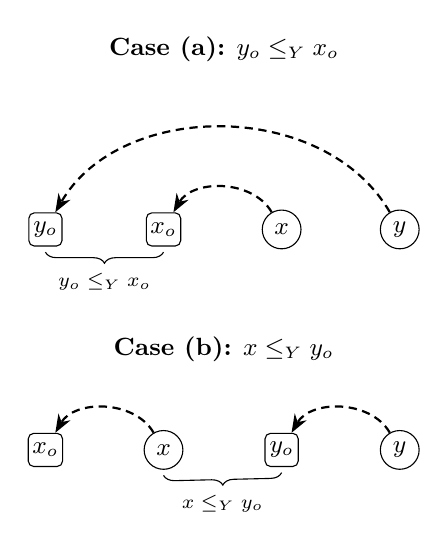
\begin{tikzpicture}[>=Stealth, every node/.style={font=\small},
             item/.style={circle, draw, inner sep=1.5pt, minimum size=14pt},
             ptr/.style={rectangle, draw, inner sep=1.5pt, minimum size=12pt,
                         rounded corners=2pt},
             origin/.style={->, thick, bend right=60, densely dashed}]
%% Case (a): y_o <= x_o  - y's origin at or left of x's origin
\begin{scope}[local bounding box=caseA]
  \node[ptr]  (yoA) at (0.0,0) {$y_o$};
  \node[ptr]  (xoA) at (1.5,0) {$x_o$};
  \node[item] (xA)  at (3.0,0) {$x$};
  \node[item] (yA)  at (4.5,0) {$y$};
  %% origin reference arrows (dashed)
  \draw[origin] (xA) to (xoA);
  \draw[origin] (yA) to (yoA);
  %% horizontal brace for y_o <= x_o
  \draw[decorate, decoration={brace, amplitude=4pt, mirror}]
    ([yshift=-2pt]yoA.south) -- ([yshift=-2pt]xoA.south)
    node[midway, below=4pt, font=\scriptsize] {$y_o \YjsLeq x_o$};
\end{scope}
\node[above=10pt] at (caseA.north) {\textbf{Case (a):} $y_o \YjsLeq x_o$};

%% Case (b): x <= y_o  - x at or left of y's origin
\begin{scope}[local bounding box=caseB, shift={(0,-2.8)}]
  \node[ptr]  (xoB) at (0.0,0) {$x_o$};
  \node[item] (xB)  at (1.5,0) {$x$};
  \node[ptr]  (yoB) at (3.0,0) {$y_o$};
  \node[item] (yB)  at (4.5,0) {$y$};
  \draw[origin] (xB) to (xoB);
  \draw[origin] (yB) to (yoB);
  \draw[decorate, decoration={brace, amplitude=4pt, mirror}]
    ([yshift=-2pt]xB.south) -- ([yshift=-2pt]yoB.south)
    node[midway, below=4pt, font=\scriptsize] {$x \YjsLeq y_o$};
\end{scope}
\node[above=10pt] at (caseB.north) {\textbf{Case (b):} $x \YjsLeq y_o$};
\end{tikzpicture}
\caption{The No-Cross-Origin lemma (Lemma~\ref{lem:no-cross-origin}).
  Items are circles, pointers (origins) are rectangles, and dashed arrows
  indicate the $\mathit{origin}$ field of each item; positions on the line
  reflect the order $\YjsLt$.  Assuming $x \YjsLt y$, either (a)~$y$'s
  origin lies at or left of $x$'s origin or (b)~$x$ itself lies at or left
  of $y$'s origin; the ``forbidden'' configuration ($y_o$ strictly between
  $x_o$ and $x$) cannot arise.}
\label{fig:no-cross-origin}
\end{figure}

\noindent
The proof uses strong induction on $|x| + |y|$; the key case
(\textsc{Lt-RightOrigin}) relies on condition~I3 to chain origin
reachability.  See Appendix~\ref{app:order-proofs} for the full proof.

%%
%% -------------------------------------------------------------------
\section{Insert Algorithm and Commutativity}
\label{sec:algorithm}
%%

%% P1: Goal is commutativity
This section establishes concurrent commutativity for Yjs: two concurrent
operations commute on every state at which they are both valid.  Splitting
on the two operation kinds, the delete-delete case is immediate because
deletion only adds to the $\mathit{deletedIds}$ component of the state and
set union is commutative; the insert-delete case is immediate because
inserts and deletes touch disjoint components of the state ($\mathit{arr}$
versus $\mathit{deletedIds}$).  The remainder of the section is devoted to
insert-insert.

The strategy is direct: we prove that Yjs insert places its new item at
the unique position that keeps $\mathit{arr}$ sorted under $\YjsLt$.  The
empty array is sorted, and both insert and delete preserve sortedness, so
the array maintained by any execution of the Yjs operations is sorted.
Two sorted arrays containing the same item set are identical, since a
strict total order admits at most one sorted arrangement of any set, so
two delivery orders that produce the same set of items produce identical
arrays.

%% P2: State Invariant
We begin with the invariant that any state reached during execution must
satisfy.  It is the state-level counterpart of the item-set invariant of
\S\ref{sec:order}, together with a pairwise-sortedness condition on the
items array.

\begin{definition}[State invariant (\leanref{YjsArrInvariant})]
\label{def:state-inv}
A state $s = (\mathit{arr}, \mathit{del})$ satisfies the \emph{Yjs array
invariant} when the following hold:
\begin{enumerate}
\item $\langle \mathit{arr} \rangle$ is a closed item set
  (Definition~\ref{def:closed-item-set}).
\item $\langle \mathit{arr} \rangle$ satisfies conditions I1--I3 of the
  item-set invariant (Definition~\ref{def:item-set-invariant}).
\item $\mathit{arr}$ is pairwise sorted by $\YjsLt$:
  for all $i < j$, $\mathit{arr}[i] \YjsLt \mathit{arr}[j]$.
\item All item identifiers in $\mathit{arr}$ are pairwise distinct.
\end{enumerate}
Here $\langle \mathit{arr} \rangle$ is the item set induced by the array,
containing $\First$, $\Last$, and each item in $\mathit{arr}$.
\end{definition}

%% P5: Item Validity
We next define the validity predicate that serves both as the
operation-network instantiation of broadcast validity~(V) and as the
precondition under which the commutativity proof operates.  The
definition has two layers.  Item validity, defined first, applies to
fully formed Yjs items and asks for the per-item analogues of conditions
I1 and I3 of the item-set invariant.  Insert-input validity, defined
second, applies to the actual operation payloads.  The two layers differ
because an insert input only carries the \emph{identifiers} of its origin
and right-origin neighbors, not the items themselves; we must first
resolve those identifiers against the current array, producing the
pointer-embedded item the input would create, before the structural
conditions on origins make sense.

\begin{definition}[Item and input validity (\leanref{IsItemValid})]
\label{def:item-valid}
An item $x = \langle o, r, \mathit{id}, c \rangle$ is \emph{valid} in a
closed item set $P$ containing $x$ together with all pointers
origin-reachable from it when:
\begin{enumerate}
\item $o \YjsLt r$;
\item for every pointer $z$ origin-reachable from $x$, either
  $z \YjsLeq o$ or $r \YjsLeq z$.
\end{enumerate}
Given an insert input $\mathit{inp}$ and a state $s$, write
$\mathit{inp}.\mathit{toItem}(s)$ for the item
$\langle o, r, \mathit{inp}.\mathit{id}, \mathit{inp}.\mathit{content}
\rangle$ in which $o$ and $r$ are obtained by looking up
$\mathit{inp}.\mathit{originId}$ and
$\mathit{inp}.\mathit{rightOriginId}$ in $s.\mathit{arr}$ (using $\First$
and $\Last$ as defaults at the boundaries).  We say $\mathit{inp}$ is
\emph{valid at $s$}, written $\mathit{inp}.\mathit{isValid}(s)$, when
$\mathit{inp}.\mathit{toItem}(s)$ is valid in
$\langle s.\mathit{arr} \rangle$; this is the predicate that instantiates
condition~(V) for Yjs.
\end{definition}

\noindent
Item validity is state-dependent: the same item may be valid at one state
but invalid at another.  Broadcast validity~(V) speaks of the state at
which the item is \emph{issued}, whereas the preservation and
commutativity theorems below need validity at the state to which the
insert is \emph{applied}.  The bridge between the two (sufficient under
causal delivery) is the \emph{causal validity} property of
\S\ref{sec:convergence}.

%% P6: Insert Preservation
We now prove that Yjs insert preserves the state invariant.

\begin{theorem}[Insert preservation (\leanref{YjsArrInvariant\_integrate})]
\label{thm:ins-pres}
If state $s$ satisfies the Yjs array invariant and an insert input
$\mathit{inp}$ is valid at $s$ (Definition~\ref{def:item-valid}), then
$\effect(\mathsf{Insert}(\mathit{inp}), s)$ also satisfies the invariant.
\end{theorem}

\noindent
The analogous preservation for deletes is trivial: deletion only modifies
$\mathit{deletedIds}$ and leaves $\mathit{arr}$ unchanged.  The proof of
insert preservation proceeds by a loop invariant on
Algorithm~\ref{alg:integrate}: we give a four-part invariant for the loop,
show that each iteration preserves it, and show that at termination the
invariant pins down the unique sorted insertion position.

%% P3: Loop Invariant
\begin{definition}[Integration invariant (\leanref{IntegrationInvariant})]
\label{def:loop-inv}
Throughout the loop of Algorithm~\ref{alg:integrate} write
$\mathit{newItem} = \mathit{inp}.\mathit{toItem}(s.\mathit{arr})$ for the
item being inserted.  The \emph{integration invariant} at iteration
position~$i$ (with candidate destination $\mathit{dest}$ and flag
$\mathit{scanning}$) asserts the following.
\begin{enumerate}
\item \textbf{Confirmed prefix} (\texttt{prefixLt}).
  For all $j < \mathit{dest}$, $\mathit{arr}[j] \YjsLt \mathit{newItem}$.
\item \textbf{Pending region} (\texttt{scannedRegion}).
  For all $\mathit{dest} \leq j < i$, one of the following holds:
  \begin{itemize}
  \item[(a)] $\mathit{arr}[j].\mathit{origin} = \mathit{newItem}.\mathit{origin}$
    and $\mathit{newItem}.\mathit{id} < \mathit{arr}[j].\mathit{id}$;
  \item[(b)] $\mathit{newItem}.\mathit{origin} \YjsLt
    \mathit{arr}[j].\mathit{origin}$.
  \end{itemize}
\item \textbf{Scanning flag} (\texttt{scanningOrigin}).
  $\mathit{scanning}$ is set exactly when
  $\mathit{arr}[\mathit{dest}].\mathit{origin} =
  \mathit{newItem}.\mathit{origin}$.
\item \textbf{Boundary ordering} (\texttt{doneLt}).
  When the loop exits via \textsc{break} at iteration $i$, we have
  $\mathit{newItem} \YjsLt \mathit{arr}[i]$.
\end{enumerate}
\end{definition}

\noindent
The loop maintains, at iteration~$i$, a partition of the array positions
$j \in [0, i)$ examined so far into a \emph{confirmed prefix}
($j < \mathit{dest}$) and a \emph{pending region}
($\mathit{dest} \leq j < i$); see Figure~\ref{fig:loop-partition}.
Confirmed-prefix elements satisfy
$\mathit{arr}[j] \YjsLt \mathit{newItem}$ (condition~1).  Pending-region
elements have not yet been ordered against $\mathit{newItem}$, but by
condition~(2) they all satisfy clause~(a) or clause~(b): clause~(a)
records that $\mathit{arr}[j]$ shares $\mathit{newItem}$'s origin while
having a larger identifier, and clause~(b) records that $\mathit{arr}[j]$
has a strictly greater origin than $\mathit{newItem}$.
Lemma~\ref{lem:pending-prop} below shows that whenever the loop
encounters a strictly larger element
$\mathit{newItem} \YjsLt \mathit{arr}[i]$, every $j$ in
$[\mathit{dest}, i)$ also satisfies
$\mathit{newItem} \YjsLt \mathit{arr}[j]$; the scanning-flag
condition~(3) is what makes that proof go through.  Combined with the
boundary ordering~(4) and the confirmed prefix, this implies that at
loop exit $\mathit{dest}$ is the smallest position at which
$\mathit{newItem} \YjsLt \mathit{arr}[\mathit{dest}]$, that is, the
unique position at which inserting $\mathit{newItem}$ preserves
pairwise sortedness.  In the remainder of this subsection we establish
that the invariant holds at loop entry and is preserved by each
iteration, and we prove Lemma~\ref{lem:pending-prop}.

\begin{figure}[t]
\centering
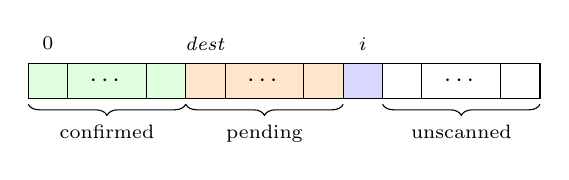
\begin{tikzpicture}
\def\rt{0.45}    % row top y
\def\rb{0}       % row bottom y
\def\lt{0.7}     % index label y (above)
%% Confirmed region: x in [0, 2]
\fill[green!12] (0,\rb) rectangle (2,\rt);
\draw (0,\rb) rectangle (2,\rt);
\draw (0.5,\rb) -- (0.5,\rt);
\draw (1.5,\rb) -- (1.5,\rt);
\node[font=\small] at (1, 0.225) {$\cdots$};
\node[font=\scriptsize] at (0.25, \lt) {$0$};
%% Pending region: x in [2, 4]
\fill[orange!20] (2,\rb) rectangle (4,\rt);
\draw (2,\rb) rectangle (4,\rt);
\draw (2.5,\rb) -- (2.5,\rt);
\draw (3.5,\rb) -- (3.5,\rt);
\node[font=\small] at (3, 0.225) {$\cdots$};
\node[font=\scriptsize] at (2.25, \lt) {$\mathit{dest}$};
%% Current cell: x in [4, 4.5]
\fill[blue!15] (4,\rb) rectangle (4.5,\rt);
\draw (4,\rb) rectangle (4.5,\rt);
\node[font=\scriptsize] at (4.25, \lt) {$i$};
%% Unscanned region: x in [4.5, 6.5]
\draw (4.5,\rb) rectangle (6.5,\rt);
\draw (5,\rb) -- (5,\rt);
\draw (6,\rb) -- (6,\rt);
\node[font=\small] at (5.5, 0.225) {$\cdots$};
%% Region braces below (current cell has no brace)
\draw[decorate, decoration={brace, amplitude=4pt, mirror}]
  ([yshift=-2pt]0,\rb) -- ([yshift=-2pt]2,\rb)
  node[midway, below=4pt, font=\scriptsize] {confirmed};
\draw[decorate, decoration={brace, amplitude=4pt, mirror}]
  ([yshift=-2pt]2,\rb) -- ([yshift=-2pt]4,\rb)
  node[midway, below=4pt, font=\scriptsize] {pending};
\draw[decorate, decoration={brace, amplitude=4pt, mirror}]
  ([yshift=-2pt]4.5,\rb) -- ([yshift=-2pt]6.5,\rb)
  node[midway, below=4pt, font=\scriptsize] {unscanned};
\end{tikzpicture}
\caption{Partition of the array positions at iteration~$i$ of
  Algorithm~\ref{alg:integrate}, with horizontal braces below
  indicating each region's extent.  The
  \emph{confirmed prefix} ($0 \leq j < \mathit{dest}$) collects
  positions already known to precede $\mathit{newItem}$ in
  $\YjsLt$; the \emph{pending region}
  ($\mathit{dest} \leq j < i$) collects positions whose ordering
  against $\mathit{newItem}$ has not yet been resolved; the cell
  at index~$i$ is the position the loop is currently examining;
  and the \emph{unscanned suffix} ($j > i$) consists of positions
  the loop has not yet visited.  Within each region only the
  leftmost cell is labeled with its starting index; intermediate
  cells are abbreviated by~$\cdots$.}
\label{fig:loop-partition}
\end{figure}

\paragraph{Initialization.}
The loop starts at $i = \mathit{leftIdx} + 1$ with
$\mathit{dest} = \mathit{leftIdx} + 1$ and
$\mathit{scanning} = \mathbf{false}$.  The confirmed prefix contains all
elements before $\mathit{leftIdx} + 1$, each $\YjsLt \mathit{newItem}$
because $\mathit{newItem}.\mathit{origin}$ sits at position
$\mathit{leftIdx}$ and the array is sorted; the pending region and
scanning flag are vacuous, and the boundary ordering condition does not
yet apply.

\paragraph{Preservation (\leanref{loopInv\_preserve1}).}
At each iteration of Algorithm~\ref{alg:integrate}, the body either
advances $\mathit{dest}$ to $i+1$ (so $\mathit{arr}[i]$ joins the
confirmed prefix), keeps $\mathit{dest}$ fixed (so $\mathit{arr}[i]$
joins the pending region), or exits the loop via \textsc{break}.  In
each case we must establish one of:
\begin{description}
\item[(a)] $\mathit{arr}[i] \YjsLt \mathit{newItem}$
  (advancing $\mathit{dest}$);
\item[(b)] either
  $\mathit{arr}[i].\mathit{origin} = \mathit{newItem}.\mathit{origin}$
  with $\mathit{newItem}.\mathit{id} < \mathit{arr}[i].\mathit{id}$, or
  $\mathit{newItem}.\mathit{origin} \YjsLt
  \mathit{arr}[i].\mathit{origin}$, together with the scanning-flag
  invariant ($\mathit{scanning} \Rightarrow
  \mathit{arr}[\mathit{dest}].\mathit{origin} =
  \mathit{newItem}.\mathit{origin}$) (extending the pending region);
\item[(c)] $\mathit{newItem} \YjsLt \mathit{arr}[i]$
  (exiting via \textsc{break}, supplying \textbf{doneLt}).
\end{description}
The branches of Algorithm~\ref{alg:integrate} divide as follows.
\begin{itemize}
\item \emph{Lines~9--10}
  ($\mathit{arr}[i].\mathit{origin}$ at an index strictly less than
  $\mathit{leftIdx}$): the loop exits and we must show~(c).
\item \emph{Lines~12--13} (same origin,
  $\mathit{newItem}.\mathit{clientId} >
  \mathit{arr}[i].\mathit{clientId}$):
  $\mathit{dest}$ advances and we must show~(a).
\item \emph{Lines~14--15} (same origin and same right-origin):
  the loop exits and we must show~(c).
\item \emph{Lines~16--17} (same origin, different right-origin):
  $\mathit{arr}[i]$ enters the pending region under clause~(2a) and we
  must show~(b).
\item \emph{Otherwise} (greater origin): when $\neg\mathit{scanning}$,
  $\mathit{dest}$ advances and we show~(a); when $\mathit{scanning}$,
  $\mathit{arr}[i]$ enters the pending region under clause~(2b) and we
  show~(b).
\end{itemize}
Each case follows from the rules of Figure~\ref{fig:yjs-order} together
with the no-cross-origin lemma (Lemma~\ref{lem:no-cross-origin}); see
Appendix~\ref{app:preservation-cases} for the detailed case analysis.

\paragraph{Postcondition.}
When the loop terminates, the invariant gives a destination~$d$ and a
loop bound~$i$ such that $\mathit{arr}[j] \YjsLt \mathit{newItem}$ for
all $j < d$ (confirmed prefix) and $\mathit{newItem} \YjsLt
\mathit{arr}[i]$ (from \textbf{doneLt} in the \textsc{break} case, and
vacuously when the loop reaches $\mathit{rightIdx}$).  The pending
region $d \leq j < i$ is collapsed onto the confirmed prefix by the
following lemma.

\begin{lemma}[Pending propagation (\leanref{pending\_propagation})]
\label{lem:pending-prop}
Suppose the integration invariant holds at position~$i$ and
$\mathit{newItem} \YjsLt \mathit{arr}[i]$.  Then $\mathit{newItem}
\YjsLt \mathit{arr}[j]$ for every $j$ with $\mathit{dest} \leq j < i$.
\end{lemma}

\noindent\textit{Proof sketch.}
By strong induction on the size of $a_j := \mathit{arr}[j]$, and a
case split on clause~(2) of Definition~\ref{def:loop-inv}.  Let
$r_1 = \mathit{newItem}.\mathit{rightOrigin}$ and
$r_2 = a_j.\mathit{rightOrigin}$.

\textbf{Case (a):}
$a_j.\mathit{origin} = \mathit{newItem}.\mathit{origin}$ and
$\mathit{newItem}.\mathit{id} < a_j.\mathit{id}$.  We apply
\textsc{Conflict-SameOrigin}, which requires
$\mathit{newItem} \YjsLt r_2$ and $a_j \YjsLt r_1$.  The second holds
because the sorted invariant places $a_j$ strictly before the array
position of $r_1$, which the loop has not yet reached.  For the first,
write $r_2 = \mathit{arr}[k]$ for some index $k > j$.  If $k < i$ then
$k$ itself lies in the pending region, so the inductive hypothesis
gives $\mathit{newItem} \YjsLt \mathit{arr}[k] = r_2$; if $i \leq k$
then $\mathit{newItem} \YjsLt \mathit{arr}[i] \YjsLeq \mathit{arr}[k]
= r_2$ by the lemma's hypothesis combined with sortedness.  In either
case, \textsc{Conflict-SameOrigin} concludes $\mathit{newItem} \YjsLt
a_j$.

\textbf{Case (b):} $\mathit{newItem}.\mathit{origin} \YjsLt
a_j.\mathit{origin}$.  By the preservation analysis above, clause~(2b)
is only ever entered while $\mathit{scanning}$ is set, so we may assume
$\mathit{scanning}$.  Condition~(3) of the invariant then gives
$\mathit{arr}[\mathit{dest}].\mathit{origin} =
\mathit{newItem}.\mathit{origin}$, and the sorted invariant gives
$\mathit{arr}[\mathit{dest}] \YjsLt a_j$.  No-cross-origin
(Lemma~\ref{lem:no-cross-origin}) upgrades this to
$\mathit{arr}[\mathit{dest}] \YjsLeq a_j.\mathit{origin}$, hence
$\mathit{newItem} \YjsLeq a_j.\mathit{origin}$, and
\textsc{Lt-Origin} closes the case.

\smallskip
\noindent
With Lemma~\ref{lem:pending-prop}, insert preservation follows: at
termination the confirmed prefix gives
$\mathit{arr}[d-1] \YjsLt \mathit{newItem}$ and pending propagation
gives $\mathit{newItem} \YjsLt \mathit{arr}[d]$, so $d$ is the unique
position at which inserting $\mathit{newItem}$ preserves pairwise
sortedness (\leanref{YjsArrInvariant\_insertIdxIfInBounds}).  The
other three parts of the invariant transfer by routine calculation.

%% P7: Insert-Insert Commutativity
We isolate as a separate lemma the structural fact that two concurrent
inserts do not disturb each other's validity, since it is the only
place where the network-level assumption~(Y1) on distinct broadcasters
enters the commutativity proof.

\begin{lemma}[Concurrent insert validity preserved]
\label{lem:conc-valid}
Let $\mathit{inp}_a$ and $\mathit{inp}_b$ be two concurrent insert
inputs broadcast in a Yjs operation network with
$\mathit{inp}_a.\mathit{clientId} \neq
\mathit{inp}_b.\mathit{clientId}$, and let $s$ satisfy the Yjs array
invariant with both $\mathit{inp}_a.\mathit{isValid}(s)$ and
$\mathit{inp}_b.\mathit{isValid}(s)$.  Then $\mathit{inp}_b$ is valid at
$\effect(\mathsf{Insert}(\mathit{inp}_a), s)$, and symmetrically with
the roles of $a$ and $b$ exchanged.
\end{lemma}

\noindent\textit{Proof.}
Distinct client identifiers~(Y1) force
$\mathit{inp}_a.\mathit{id} \neq \mathit{inp}_b.\mathit{id}$, so the
items $\mathit{inp}_a.\mathit{toItem}(s)$ and
$\mathit{inp}_b.\mathit{toItem}(s)$ have distinct identifiers.  By
Theorem~\ref{thm:ins-pres}, inserting the $a$-item leaves the array
invariant intact, and the resulting array contains every item of
$s.\mathit{arr}$ together with the $a$-item.  All ancestors of
$\mathit{inp}_b.\mathit{toItem}$, in particular those that resolve its
$\mathit{originId}$ and $\mathit{rightOriginId}$, remain present, so
$\mathit{inp}_b.\mathit{toItem}$ resolves to the same item against the
larger array, and the per-item validity conditions of
Definition~\ref{def:item-valid} continue to hold.

\begin{corollary}[Insert-insert commutativity, \leanref{integrate\_ok\_commutative}]
\label{thm:ins-ins}
Let $s$ satisfy the Yjs array invariant and let $a$, $b$ be two
concurrent insert inputs broadcast in a Yjs operation network with
$a.\mathit{clientId} \neq b.\mathit{clientId}$, both valid at $s$.
Then
\[
  \effect(\mathsf{Insert}(a), \effect(\mathsf{Insert}(b), s)) =
  \effect(\mathsf{Insert}(b), \effect(\mathsf{Insert}(a), s)).
\]
\end{corollary}

\noindent\textit{Proof.}
By Lemma~\ref{lem:conc-valid} applied symmetrically, the operation
applied second is still valid at the post-state of the first, so
Theorem~\ref{thm:ins-pres} produces invariant-satisfying arrays in both
orders.  These arrays contain the same underlying item set (the items
of $s$ together with the items induced by $a$ and $b$) and the
invariant requires pairwise sortedness by $\YjsLt$.  Since $\YjsLt$ is
a strict total order on invariant-satisfying item sets
(Theorems~\ref{thm:totality}--\ref{thm:asymmetry}), the two sorted
arrays are identical (\leanref{same\_yjs\_set\_unique}).

\smallskip
\noindent
Corollary~\ref{thm:ins-ins} is the concurrent-commutativity statement we
need, but its hypothesis appeals to item validity at $s$ for both
inserts, whereas the operation-network axiom~(V) only guarantees
validity at the state at which each insert was \emph{broadcast}.
Section~\ref{sec:convergence} closes this gap by showing that under
causal delivery broadcast-time validity transports to any state whose
delivery list contains the insert's $\hb$-predecessors, lifting
Corollary~\ref{thm:ins-ins} to the conditional concurrent commutativity
premise of the generic convergence theorem.

%%
%% -------------------------------------------------------------------
\section{Convergence}
\label{sec:convergence}
%%

This section instantiates the generic convergence framework of
\S\ref{subsec:our-approach} for Yjs.  We take $S$ to be the set of
insert and delete messages broadcast by some node, $\Phi$ to be the
Yjs state invariant (Definition~\ref{def:state-inv}), and
$\mathit{isValid}$ to be the input validity predicate
$\mathit{inp}.\mathit{isValid}(s)$ of
Definition~\ref{def:item-valid}.  With these definitions, the
state-invariant preservation clause of
Definition~\ref{def:causally-valid} is exactly
Theorem~\ref{thm:ins-pres}, and the two substantial premises, causal
validity and conditional concurrent commutativity, are established by
the two lemmas below.

\begin{lemma}[Yjs causal validity (\leanref{isValidState\_insert\_causally})]
\label{lem:yjs-causal-valid}
The Yjs operation network is causally validatable
(Definition~\ref{def:causally-valid}) with source set the messages
broadcast by some node, with $\mathit{isValid}$ taken to be the
input-validity predicate of Definition~\ref{def:item-valid}.
\end{lemma}

\noindent\textit{Proof sketch.}
Broadcast validity~(V) gives, for each source $a$, a state $s^\star$ at
which $a$ is valid: the local state at the broadcasting replica just
before the broadcast.  Let $L$ be any $\hb$-consistent, $\hb$-closed,
duplicate-free list containing every $\hb$-predecessor of $a$, and let
$s = \interpOps(L, \init)$.  We transport input validity from $s^\star$
to $s$ in two steps.  First, every item present at $s^\star$ is also
present at $s$: by broadcast validity the $\hb$-predecessors of $a$
populate $s^\star$, and they are all contained in $L$ by assumption,
while the items array is monotone under insert and delete.  Second,
input validity depends only on which items are origin-reachable from
$a.\mathit{toItem}$, not on their positions within the sorted array,
and Theorem~\ref{thm:ins-pres} ensures that $s$ satisfies the array
invariant.

We next show that the delivered operations at any node form a list
satisfying conditional concurrent commutativity.  Corollary
\ref{thm:ins-ins} already establishes the insert-insert case for two
concurrent inserts with distinct client identifiers and both valid at
the current state; the lemma below puts the remaining pieces together.

\begin{lemma}[Yjs conditional concurrent commutativity,
  \leanref{YjsOperationNetwork\_concurrentCommutative}]
\label{thm:yjs-comm}
The delivered messages of any Yjs operation network satisfy
conditional concurrent commutativity (Definition~\ref{def:conditional-comm})
with respect to the Yjs array invariant and input validity.
\end{lemma}

\noindent\textit{Proof sketch.}
By a case analysis on the operation kinds of the concurrent pair.  The
delete-delete and insert-delete cases are immediate from the
disjointness of $\mathit{arr}$ and $\mathit{deletedIds}$, as discussed
at the start of \S\ref{sec:algorithm}.  For the insert-insert case
Corollary~\ref{thm:ins-ins} applies once we discharge its two missing
hypotheses: $a.\mathit{clientId} \neq b.\mathit{clientId}$ and that
$a$, $b$ are not origin-reachable from each other.  The first follows
because two concurrent broadcasts come from different broadcasters,
which by~(Y1) means different client identifiers.  The second follows
from causal validity (Lemma~\ref{lem:yjs-causal-valid}): any item
origin-reachable from $a$'s would have to be present already at the
broadcast state of $a$, but a concurrent operation $b$ is by
definition not in $a$'s broadcast prefix; the detailed proof is
deferred to Appendix~\ref{app:not-reach}.

%% P7: Yjs Convergence
Combining the two lemmas with the structural causal-network premises
yields the main convergence result.

\begin{theorem}[Yjs Convergence (\leanref{YjsOperationNetwork\_converge'})]
\label{thm:yjs-convergence}
For any Yjs operation network, if nodes $i$ and $j$ deliver the same
set of operations ($\Delivered{i}(H_i) \approx \Delivered{j}(H_j)$),
then
$\interpOps(\Delivered{i}(H_i), \init) =
 \interpOps(\Delivered{j}(H_j), \init)$.
\end{theorem}

\noindent\textit{Proof.}
Apply Theorem~\ref{thm:generic-conv} to
$L_0 = \Delivered{i}(H_i)$ and $L_1 = \Delivered{j}(H_j)$.  Causal
validity and conditional concurrent commutativity are
Lemmas~\ref{lem:yjs-causal-valid} and~\ref{thm:yjs-comm}; the
remaining structural hypotheses ($\hb$-consistency, $\hb$-closedness,
and duplicate-freedom of $\Delivered{i}(H_i)$ and
$\Delivered{j}(H_j)$) follow from the causal-network axioms (N1--N3)
together with the order-preservation of causal delivery.

%%
%% -------------------------------------------------------------------
\section{Related Work}
\label{sec:related}
%%

%% P1: Shapiro-style op-based CRDTs
Shapiro et al.~\cite{Shapiro2011} formulate operation-based CRDTs in terms
of \emph{enabled} effectors: an effector is enabled only on states for
which a delivery precondition $P$ holds, and concurrent commutativity is
required only between effectors enabled at a common reachable state, with
the additional obligation that applying one effector preserves the
enabledness of the other.  The op-based CRDT theorem then asks that causal
delivery satisfy~$P$, allowing the system to delay delivery until the
precondition is met.  Our work should not be read as introducing
delivery preconditions to CRDT theory; rather, we give a prefix-level
formulation of the same readiness obligation, written as an invariant on
$\hb$-consistent, $\hb$-closed prefixes, and use it to mechanize a
swap-based convergence theorem.

%% P2: Matrix Event Graph
Jacob et al.~\cite{MatrixEventGraph2022} analyse the Matrix Event Graph as
a CRDT in the Shapiro framework and give a concrete proof of its delivery
precondition: they prove that $P$ is preserved by the application of
later operations, use that preservation in their commutativity proof,
and observe that causal delivery immediately satisfies $P$ on reception
because the parent vertices of an event are never removed.  This is close
in spirit to the prefix-level causal validity condition of
Definition~\ref{def:causally-valid}.  The difference is that we abstract
the obligation into a reusable convergence theorem and instantiate it for
the more state-dependent Yjs insertion algorithm, whose commutativity
depends on a recursively defined structural order rather than on the
relatively uniform parent/child relation of an event graph.

%% P3: Gomes et al. and other mechanized CRDT theories
Gomes et al.~\cite{Gomes2017,GomesRGA2017} developed a mechanized
Isabelle/HOL framework for proving strong eventual consistency and
applied it to RGA.  Their network model contains an explicit
valid-message / valid-behaviour condition; in our terminology this
corresponds to broadcast-time validity (V) of
Definition~\ref{def:operation-network}.  Their convergence theorem,
however, is based on \emph{unconditional} commutativity of concurrent
operations, so the proof does not require showing that an operation
remains valid at each intermediate reordered state.  Validity is therefore not
absent from the Gomes framework (it is present at the network level) but
their proof has no need for a prefix-level validity transport condition
because the CRDTs they verify (notably RGA, which orders concurrent
insertions via globally unique timestamps without reference to the
current state) commute unconditionally.  Yjs violates unconditional
commutativity because its insert effector is meaningful only on states
satisfying a structural invariant.  Our framework keeps the network-level
validity discipline of Gomes et al.\ but adds a prefix-level causal
validity transport condition, allowing a swap proof to proceed for
state-dependent effectors; in this sense our generic theorem refines
theirs by replacing unconditional commutativity with the pair
(conditional commutativity, prefix-level causal validity).

Zeller et al.~\cite{Zeller2014} formalize CRDTs in Coq, and
Lim and Kim~\cite{Lim2019} develop a mechanized CRDT theory; neither
addresses the Yjs/YATA family.  Other sequence CRDTs have been verified
in restricted settings~\cite{Netzell2020}.

%% P4: Fugue
Weidner et al.~\cite{Weidner2023} design the \emph{Fugue} sequence CRDT
and, in its appendix, provide a by-hand proof for a variant of the Yjs
insert algorithm.  Their development does not isolate conditional
commutativity as an explicit property, nor does it formulate a
prefix-level causal validity condition; instead, the proof implicitly
relies on the fact that concurrent operations originating at causally
adjacent states preserve an invariant analogous to ours, which is
precisely the content of conditional commutativity.  To the best of our
understanding of the by-hand appendix, that reliance surfaces in the
step showing that the insert procedure lands at the unique sorted position,
where the reasoning appeals to well-formedness of the current
document, a property that holds only on reachable states.  Making this
reliance explicit and machine-checked is one of the contributions of the
present paper.

%% P2: YATA paper and the bug
Nicolaescu et al.~\cite{Nicolaescu2016} introduce the YATA algorithm that
Yjs implements, with proofs sketched for a subset of the required
properties.  As discussed in \S\ref{sec:intro}, we discovered while
formalizing the algorithm that the published pseudocode admits a
non-convergent execution; the original author confirmed the issue.  Our
work provides the first complete machine-checked proof of the algorithm as
implemented in Yjs.

%% P3: Other sequence CRDTs
Other sequence CRDTs such as RGA~\cite{Roh2011} and Logoot~\cite{Weiss2010}
achieve unconditional commutativity by construction: RGA uses unique timestamps,
Logoot uses dense position identifiers.  Yjs's origin/right-origin encoding
creates structural dependencies on the existing document, which is the source
of both its expressiveness and the need for conditional commutativity.
The Attiya et al.~\cite{Attiya2016} specification work captures semantic
requirements for sequence CRDTs but does not mechanize proofs.

%%
%% -------------------------------------------------------------------
\section{Discussion and Conclusion}
\label{sec:conclusion}
%%

%% P1: Summary
We have introduced a prefix-level conditional commutativity convergence
framework that refines the unconditional-commutativity approach used by
existing mechanized CRDT theories, and instantiated it for Yjs to obtain
the first complete machine-checked proof of strong eventual consistency
for the Yjs core CRDT algorithm.  The main theorem
(\leanref{YjsOperationNetwork\_converge'}) is fully machine-checked in
Lean~4 with no axioms beyond those of its type theory.

%% P2: Conditional commutativity as a reusable framework
The framework is independent of Yjs: any CRDT whose effectors commute on
invariant-satisfying reachable states, rather than on all states, which fits
naturally into our generic theorem (Theorem~\ref{thm:generic-conv}).
Other CRDTs, such as the Matrix Event Graph~\cite{MatrixEventGraph2022},
already require reasoning about delivery preconditions and their
preservation; what appears specific to Yjs is the interaction between
such prefix-level validity transport and a non-trivial sequence insert
procedure whose commutativity depends on a recursively defined
structural order.  Identifying further CRDTs whose verification benefits
from the prefix-level formulation, and integrating it with the
Shapiro-style operational delivery-precondition discipline at the network
layer, is a direction for future work.

%% P3: Limitations and future work
The present formalization models the core CRDT algorithm with insert and
delete operations.  We do not model garbage collection, undo/redo,
subdocuments, or the awareness protocol.  The artifact contains an
incomplete indirect variant where items reference origins by identifier.
Extending the proof to these features is future work.

\bibliographystyle{ACM-Reference-Format}
\bibliography{refs}

\appendix

%%
%% -------------------------------------------------------------------
\section{Proofs of Theorems in Section~\ref{sec:order}}
\label{app:order-proofs}
%%

This appendix gives detailed proof sketches for the totality,
transitivity, and asymmetry theorems and the no-cross-origin lemma of
\S\ref{sec:order}.

\subsection{Totality}

\noindent\textit{Proof sketch} (Theorem~\ref{thm:totality}).
By strong induction on $|x| + |y|$.
The cases involving $\First$ or $\Last$ are immediate
by \textsc{Lt-First} or \textsc{Lt-Last}.  When both are items
$x = \langle x_o, x_r, \mathit{id}_x, c_x \rangle$ and
$y = \langle y_o, y_r, \mathit{id}_y, c_y \rangle$,
the proof attempts four recursive comparisons on
interval boundaries, each well-founded because
$|x_o|, |x_r| < |x|$ and $|y_o|, |y_r| < |y|$:
\begin{enumerate}
\item $x$ vs.\ $y_o$: if $x \YjsLeq y_o$, then
  $x \YjsLt y$ by \textsc{Lt-Origin}.
\item $y_r$ vs.\ $x$: if $y_r \YjsLeq x$, then
  $y \YjsLt x$ by \textsc{Lt-RightOrigin}.
\item $y$ vs.\ $x_o$: if $y \YjsLeq x_o$, then
  $y \YjsLt x$ by \textsc{Lt-Origin}.
\item $x_r$ vs.\ $y$: if $x_r \YjsLeq y$, then
  $x \YjsLt y$ by \textsc{Lt-RightOrigin}.
\end{enumerate}
If all four fail (i.e.\ $y_o \YjsLt x$, $x \YjsLt y_r$,
$x_o \YjsLt y$, $y \YjsLt x_r$), then $x$ and $y$
compete for the same interval, and a fifth comparison
on the origins decides via the conflict rules:
if $x_o \neq y_o$, \textsc{Conflict-DiffOrigin}
applies; if $x_o = y_o$, the ID comparison
$\mathit{id}_x$ vs.\ $\mathit{id}_y$ resolves the
tie via \textsc{Conflict-SameOrigin}; if
$\mathit{id}_x = \mathit{id}_y$, condition~I2
(ID uniqueness) forces $x = y$.

\subsection{Transitivity}

\begin{lemma}[Conflict transitivity
  (\leanref{conflict\_lt\_trans})]
\label{lem:conflict-lt-trans}
If $x \YjsLt y$ and $y \YjsLt z$ are both derived by a conflict rule
(\textsc{Conflict-DiffOrigin} or \textsc{Conflict-SameOrigin}), then
$x \YjsLt z$, assuming the transitivity inductive hypothesis holds for
all triples with total size smaller than $|x|+|y|+|z|$.
\end{lemma}
\noindent\textit{Proof sketch.}
From the two conflict derivations, the IH yields
$x_o \YjsLt z$ (since $|x_o| < |x|$) and
$x \YjsLt z_r$ (since $|z_r| < |z|$).
Totality then tests whether $x_r \YjsLeq z$ or
$x \YjsLeq z_o$; if either holds,
\textsc{Lt-RightOrigin} or \textsc{Lt-Origin} closes
the goal.  When both fail, $x$ and $z$ compete for
the same interval, and the four combinations of
\textsc{Conflict-DiffOrigin}/\textsc{Conflict-SameOrigin}
resolve via the conflict rules (in the
\textsc{DiffOrigin}~$\times$~\textsc{DiffOrigin} case,
a further IH on the origins produces $z_o \YjsLt x_o$;
the remaining three cases apply a conflict rule
directly).

\medskip
\noindent\textit{Proof sketch} (Theorem~\ref{thm:transitivity}).
By strong induction on $|x| + |y| + |z|$.
A case-analysis lemma (\leanref{yjs\_lt\_cases})
decomposes each $\YjsLt$ derivation into
\textsc{Lt-RightOrigin}, \textsc{Lt-Origin}, or one
of the conflict rules
(\textsc{Conflict-DiffOrigin}/\textsc{Conflict-SameOrigin}).
The proof handles all nine combinations of
derivation rules for $x \YjsLt y$ and $y \YjsLt z$.

\smallskip\noindent\textbf{$x \YjsLt y$ by \textsc{Lt-RightOrigin}
($x_r \YjsLeq y$):}
This case is uniform in $y \YjsLt z$.
If $x_r = y$, substitute directly.
If $x_r \YjsLt y$, the IH on $(x_r, y, z)$
applies because $|x_r| < |x|$;
then \textsc{Lt-RightOrigin} gives $x \YjsLt z$.

\smallskip\noindent\textbf{$x \YjsLt y$ by \textsc{Lt-Origin}
($x \YjsLeq y_o$):}
We sub-case on $y \YjsLt z$.

\begin{itemize}
\item \emph{$y \YjsLt z$ by \textsc{Lt-RightOrigin}
  ($y_r \YjsLeq z$)}:
  By I1, $y_o \YjsLt y_r$.  We must chain
  $x \YjsLeq y_o \YjsLt y_r \YjsLeq z$,
  but transitivity is not yet established.
  The key observation is that the IH is on
  $|x|+|y|+|z|$, and since
  $|y_o|+|y_r|+2 = |y|$ we have
  $|x|+|y_o|+|y_r| < |x|+|y| \le |x|+|y|+|z|$,
  so the IH applies to the triple $(x, y_o, y_r)$
  to give $x \YjsLt y_r$.  Then
  $x \YjsLt z$ follows from the IH on
  $(x, y_r, z)$ since $|y_r| < |y|$.

\item \emph{$y \YjsLt z$ by \textsc{Lt-Origin}
  ($y \YjsLeq z_o$)}:
  It suffices to show $x \YjsLt z_o$
  (then \textsc{Lt-Origin} gives $x \YjsLt z$).
  If $y = z_o$, we have $x \YjsLt y = z_o$.
  If $y \YjsLt z_o$, the IH on $(x, y, z_o)$
  applies because $|z_o| < |z|$.

\item \emph{$y \YjsLt z$ by a conflict rule}:
  A helper lemma extracts
  $y_o \YjsLt z$ from any conflict derivation
  of $y \YjsLt z$.  Then
  $x \YjsLeq y_o \YjsLt z$;
  the IH on $(x, y_o, z)$ applies because
  $|y_o| < |y|$.
\end{itemize}

\noindent\textbf{$x \YjsLt y$ by a conflict rule:}
A helper lemma extracts $x \YjsLt y_r$ from any
conflict derivation of $x \YjsLt y$.
When $y \YjsLt z$ by \textsc{Lt-RightOrigin}
($y_r \YjsLeq z$), the IH on $(x, y_r, z)$ applies
since $|y_r| < |y|$.
When $y \YjsLt z$ by \textsc{Lt-Origin}
($y \YjsLeq z_o$), we reduce to showing
$x \YjsLt z_o$ and apply the IH on $(x, y, z_o)$
since $|z_o| < |z|$.
When both use a conflict rule, we apply
Lemma~\ref{lem:conflict-lt-trans}.

\subsection{Asymmetry}

\noindent\textit{Proof sketch} (Theorem~\ref{thm:asymmetry}).
By strong induction on $|x| + |y|$, assuming $x \YjsLt y$
and $y \YjsLt x$ for contradiction.
The proof decomposes each derivation via
\leanref{yjs\_lt\_cases}.
If $x \YjsLt y$ was derived by \textsc{Lt-RightOrigin}
($x_r \YjsLeq y$), a dedicated reduction lemma
shows there exist $x', y' \in P$ with
$|x'| + |y'| < |x| + |y|$ and $x' \YjsLt y'$,
$y' \YjsLt x'$, contradicting the IH.
The case for \textsc{Lt-Origin} is symmetric.
When both sides use a conflict rule,
a third reduction lemma
(\leanref{yjs\_lt\_conflict\_lt\_decreases})
similarly produces a smaller contradictory pair.

\subsection{No-Cross-Origin}

\noindent\textit{Proof sketch} (Lemma~\ref{lem:no-cross-origin}).
By strong induction on $|x| + |y|$.
The \textsc{Lt-Origin} case ($x \YjsLeq y_o$) yields
the right disjunct directly.
The conflict-rule case reads off
$y_o \YjsLt x_o$ from the conflict premises and
yields the left disjunct.
The key case is \textsc{Lt-RightOrigin}
($x_r \YjsLeq y$).  If $x_r = y$ then condition~I3
(origin reachability) gives $y_o \YjsLeq x_o$
directly.  If $x_r \YjsLt y$, the IH applies
(since $|x_r| < |x|$) to obtain either
$y_o \YjsLeq x_r.\mathit{origin}$ or
$x_r \YjsLeq y_o$; in the former branch, I3 again
chains $x_r.\mathit{origin} \YjsLeq x_o$ to produce
$y_o \YjsLeq x_o$.

%%
%% -------------------------------------------------------------------
\section{Integration Preservation: Detailed Cases}
\label{app:preservation-cases}
%%

Let $u = \mathit{newItem}$ and $o = \mathit{arr}[i]$ be the scanned element.

\begin{itemize}
\item \emph{$o.\mathit{origin} < u.\mathit{origin}$} ---
  loop exits via \textsc{break}.
  Obligation: \textbf{doneLt} ($u \YjsLt o$).
  By totality either $u \YjsLt o$ or $o \YjsLeq u$.
  If $o \YjsLt u$, Lemma~\ref{lem:no-cross-origin} yields
  $u.\mathit{origin} \YjsLeq o.\mathit{origin}$ or
  $o \YjsLeq u.\mathit{origin}$;
  the first contradicts $o.\mathit{origin} < u.\mathit{origin}$,
  the second contradicts $o$'s position past~$u.\mathit{origin}$
  in the sorted array.

\item \emph{$o.\mathit{origin} = u.\mathit{origin}$,
  $o.\mathit{id} < u.\mathit{id}$} ---
  $\mathit{dest} \leftarrow i{+}1$,
  $\mathit{scanning} \leftarrow \mathbf{false}$.
  Obligation: \textbf{prefixLt} for the expanded
  prefix~$[0, i{+}1)$.
  For each $j$ in $[\mathit{dest}, i]$:
  $\mathit{arr}[j] \YjsLeq o$ holds by the sorted array, and
  $o \YjsLt u$ by \textsc{Conflict-SameOrigin}
  (same origin, smaller ID).
  Transitivity gives $\mathit{arr}[j] \YjsLt u$.

\item \emph{Same origin, $o.\mathit{id} \geq u.\mathit{id}$,
  same right-origin} ---
  loop exits via \textsc{break}.
  Obligation: \textbf{doneLt} ($u \YjsLt o$).
  Both items share origin and right-origin with
  $u.\mathit{id} \leq o.\mathit{id}$;
  \textsc{Conflict-SameOrigin} gives $u \YjsLt o$.

\item \emph{Same origin, $o.\mathit{id} \geq u.\mathit{id}$,
  different right-origin} ---
  $\mathit{scanning} \leftarrow \mathit{true}$.
  Obligation: \textbf{scannedRegion} for~$o$.
  Condition~(2a) holds:
  $o.\mathit{origin} = u.\mathit{origin}$
  and $u.\mathit{id} < o.\mathit{id}$
  (by unique-ID distinctness).

\item \emph{$o.\mathit{origin} > u.\mathit{origin}$,
  $\neg\mathit{scanning}$} ---
  $\mathit{dest} \leftarrow i{+}1$.
  Obligation: \textbf{prefixLt} for the expanded prefix.
  When $\mathit{scanning}$ is false, $\mathit{dest}$
  equals the current scan position, so every element
  in the old pending region was already confirmed.
  The origin of~$o$ lies at some array index
  $k < \mathit{dest}$, so $o.\mathit{origin} \YjsLt u$
  by the prefix condition.
  Combined with item validity ($o$ lies between
  $u.\mathit{origin}$ and $u.\mathit{rightOrigin}$),
  we obtain $o \YjsLt u$; transitivity
  extends to all $j \leq i$.

\item \emph{$o.\mathit{origin} > u.\mathit{origin}$,
  $\mathit{scanning}$} ---
  continue; extend pending region.
  Obligation: \textbf{scannedRegion},
  condition~(2b), which asks for
  $u.\mathit{origin} \YjsLt o.\mathit{origin}$.
  This is the scan hypothesis directly.
\end{itemize}

%%
%% -------------------------------------------------------------------
\section{Concurrent Inserts Are Not Origin-Reachable}
\label{app:not-reach}
%%

This appendix supplies the proof omitted from the sketch of
Lemma~\ref{thm:yjs-comm}: in a Yjs operation network, two concurrent
insert inputs $a$ and $b$ that are both valid at a state $s$
satisfying the array invariant cannot be origin-reachable from each
other.

Let $a$ be broadcast at the state $s_a^\star$ (the local state of $a$'s
broadcaster just before the broadcast), with $a.\mathit{toItem}(s_a^\star)$
valid in $\langle s_a^\star.\mathit{arr} \rangle$ by broadcast
validity~(V).  In particular, every pointer origin-reachable from
$a.\mathit{toItem}(s_a^\star)$ is already an element of
$s_a^\star.\mathit{arr}$ (origin reachability would otherwise leave the
closed item set).  Since $a$ and $b$ are concurrent, $b$ is not in
the broadcast prefix of $a$ at $s_a^\star$, so $b$'s item does not
appear in $s_a^\star.\mathit{arr}$ and is therefore not
origin-reachable from $a$'s item.  By symmetry, $a$'s item is not
origin-reachable from $b$'s item.  These are exactly
the additional preconditions required by Corollary~\ref{thm:ins-ins}
for the items induced by $a$ and $b$ at $s$.

\end{document}
